\chapter{The Wilson-Fisher Fixed Point and Scaling Operators}
\label{ch:volume-ii-wilson-fisher-fixed-point-scaling-operators}

\section{Scalar Quartic Theory Below Four Dimensions}

The trace identity makes fixed points structurally important.  The next task is
to exhibit a non-Gaussian fixed point in a controlled calculation.  Consider a
single real scalar field in
\[
  D=4-\epsilon
\]
Euclidean dimensions, where \(\epsilon>0\) is treated as a small fixed
parameter rather than as a regulator to be removed at the end.  The bare
Lagrangian is
\[
  \mathcal L_E
  =
  \frac12\partial_\mu\phi\,\partial^\mu\phi
  +
  \frac12m_0^2\phi^2
  +
  \frac1{4!}g_0\phi^4 .
\]
The quartic coupling \(g_0\) has mass dimension \(\epsilon\).  The mass
parameter \(m_0^2\) must be tuned so that the infrared two-point function has
no mass gap.  This tuning is an infrared condition: it is not guaranteed by
the algebra of counterterms, and it is meaningful only when the flow reaches a
massless long-distance theory.

Define a dimensionless 1PI quartic coordinate by the symmetric Euclidean
subtraction condition
\[
  \lambda(\mu)
  =
  -\mu^{-\epsilon}Z(\mu)^2\,
  \Gamma^{(4)}
  \bigg|_{k_i^2=\mu^2,\;s=t=u=-\frac43\mu^2},
\]
where
\[
  Z(\mu)
  =
  \left(
    1-\frac{\partial\Sigma}{\partial k^2}
  \right)^{-1}_{k^2=\mu^2}.
\]
At one loop \(Z(\mu)=1\), and the bubble graph gives
\[
  \lambda(\mu)
  =
  \mu^{-\epsilon}
  \left[
    g_0
    -
    \frac32g_0^2(4\pi)^{-2+\epsilon/2}
    \frac{\Gamma(\epsilon/2)\Gamma(1-\epsilon/2)^2}{\Gamma(2-\epsilon)}
    \left(\frac43\mu^2\right)^{-\epsilon/2}
    +
    O(g_0^3)
  \right].
\]
Differentiating with respect to \(\log\mu\), and then expressing \(g_0\) in
terms of \(\lambda(\mu)\), gives
\[
  \frac{\dd\lambda}{\dd\log\mu}
  =
  -\epsilon\lambda
  -
  \epsilon\lambda^2
  \left[
    -\frac32(4\pi)^{-2+\epsilon/2}
    \frac{\Gamma(\epsilon/2)\Gamma(1-\epsilon/2)^2}{\Gamma(2-\epsilon)}
    \left(\frac43\right)^{-\epsilon/2}
  \right]
  +
  O(\lambda^3).
\]
Since
\[
  -\frac32(4\pi)^{-2+\epsilon/2}
  \frac{\Gamma(\epsilon/2)\Gamma(1-\epsilon/2)^2}{\Gamma(2-\epsilon)}
  \left(\frac43\right)^{-\epsilon/2}
  =
  -\frac{3}{16\pi^2}\frac1{\epsilon}+O(\epsilon^0),
\]
the beta function is
\[
  \beta(\lambda)
  =
  \frac{\dd\lambda}{\dd\log\mu}
  =
  -\epsilon\lambda
  +
  \left(\frac{3}{16\pi^2}+O(\epsilon)\right)\lambda^2
  +
  O(\lambda^3).
\]
The zero of this beta function is
\[
  \lambda_*
  =
  \frac{16\pi^2}{3}\epsilon+O(\epsilon^2).
\]
For sufficiently small \(\epsilon\), the fixed point lies in the perturbative
domain.

\begin{figure}[H]
  \centering
  \resizebox{0.98\textwidth}{!}{%
  \begin{tikzpicture}[x=1cm,y=1cm,every node/.style={font=\scriptsize}]
    \begin{scope}
      \node[font=\small, align=center] at (0,2.45)
        {quartic coordinate from a symmetric\\Euclidean 1PI vertex};
      \fill[gray!18, draw=black, thick] (0,0.45) circle (0.52);
      \node at (0,0.45) {1PI};
      \foreach \a/\lab in {35/\(k_1\),145/\(k_2\),215/\(k_3\),325/\(k_4\)} {
        \draw[thick] ({0.52*cos(\a)},{0.45+0.52*sin(\a)})
          --++({1.05*cos(\a)},{1.05*sin(\a)});
        \node at ({1.85*cos(\a)},{0.45+1.85*sin(\a)}) {\lab};
      }
      \node[align=center, blue!70!black] at (0,-1.25)
        {\(\lambda(\mu)=-\mu^{-\epsilon}Z(\mu)^2\Gamma^{(4)}\)\\
         \(k_i^2=\mu^2,\quad s=t=u=-4\mu^2/3\)};
    \end{scope}

    \begin{scope}[shift={(6.7,0)}]
      \node[font=\small, align=center] at (0,2.45)
        {flow for decreasing \(\mu\)};
      \draw[-{Latex[length=2mm]}, thick] (-3.0,0)--(3.45,0) node[below] {\(\lambda\)};
      \fill[black] (-2.25,0) circle (2pt);
      \node[below] at (-2.25,-0.08) {\(0\)};
      \fill[purple!80!black] (0.35,0) circle (2.5pt);
      \node[purple!80!black, below] at (0.35,-0.08) {\(\lambda_*\)};
      \foreach \x in {-1.75,-1.05,-0.35} {
        \draw[-{Latex[length=2mm]}, red!75!black, very thick] (\x,0.32)--++(0.52,0);
      }
      \foreach \x in {1.45,2.15,2.85} {
        \draw[-{Latex[length=2mm]}, blue!75!black, very thick] (\x,0.32)--++(-0.52,0);
      }
      \node[red!75!black] at (-1.05,1.05) {\(\beta<0\)};
      \node[blue!75!black] at (2.15,1.05) {\(\beta>0\)};
      \node[purple!80!black, align=center] at (0.35,-1.05)
        {infrared-attractive\\interacting fixed point};
    \end{scope}
  \end{tikzpicture}
  }
  \caption{The dimensionless quartic coordinate is defined by a symmetric 1PI
  subtraction.  In \(4-\epsilon\) dimensions the classical term
  \(-\epsilon\lambda\) and the one-loop term \(3\lambda^2/(16\pi^2)\) balance
  at the nonzero fixed point \(\lambda_*\).}
  \label{fig:volume-ii-wilson-fisher-flow}
\end{figure}

The bare coupling and the renormalized coupling have different infrared
behavior.  The naive dimensionless bare combination \(\mu^{-\epsilon}g_0\)
diverges as \(\mu\to0\).  The renormalized coupling \(\lambda(\mu)\), after the
fluctuation correction in the 1PI coordinate definition is included, approaches
the finite value \(\lambda_*\) along the massless critical trajectory.

\begin{figure}[H]
  \centering
  \resizebox{0.85\textwidth}{!}{%
  \begin{tikzpicture}[x=1cm,y=1cm,every node/.style={font=\scriptsize}]
    \draw[-{Latex[length=2mm]}, thick] (-3.2,0)--(3.5,0) node[below] {\(\mu\downarrow0\)};
    \node[align=center] at (-1.8,1.78)
      {naive coordinate\\\(\mu^{-\epsilon}g_0\to\infty\)};
    \draw[red!75!black, very thick, -{Latex[length=2mm]}]
      (-2.55,0.32)..controls (-1.8,0.72) and (-1.05,1.02)..(-0.2,1.28);
    \node[align=center] at (1.55,1.45)
      {1PI coordinate\\\(\lambda(\mu)\to\lambda_*\)};
    \draw[blue!75!black, very thick, -{Latex[length=2mm]}]
      (0.15,0.35)..controls (0.95,0.72) and (1.75,0.78)..(2.55,0.78);
    \draw[purple!80!black, dashed] (2.55,0.05)--(2.55,1.0);
    \node[purple!80!black, right] at (2.55,0.78) {\(\lambda_*\)};
  \end{tikzpicture}
  }
  \caption{The finite infrared coupling is a property of the renormalized 1PI
  coordinate, not of the naive dimensionless bare coupling.}
  \label{fig:volume-ii-naive-versus-renormalized-coupling}
\end{figure}

\section{The First Scaling Operators}

At a fixed point, the anomalous-dimension matrix can be diagonalized into
scaling operators.  The elementary field \(O_1=\phi\) has anomalous dimension
\[
  \gamma_\phi
  =
  \frac12\frac{\dd\log Z(\mu)}{\dd\log\mu}.
\]
Since \(Z(\mu)=1+O(\lambda^2)\) in scalar quartic theory, the field anomalous
dimension starts only at order \(\lambda_*^2=O(\epsilon^2)\).  Thus
\[
  \Delta_\phi
  =
  \frac{D-2}{2}+\gamma_{\phi*}
  =
  1-\frac{\epsilon}{2}+O(\epsilon^2).
\]

The operator \(O_2=\phi^2\) is more delicate.  The constant source deformation
\[
  \delta S=\int\dd^D x\,\delta g_2\,\phi^2(x)
\]
corresponds to a zero-momentum insertion.  In the massless theory, the
one-loop graph then contains an infrared-divergent integral of the form
\[
  \int\frac{\dd^D\ell}{(2\pi)^D}\,\frac{1}{(\ell^2)^2}.
\]
The divergence is caused by the subtraction kinematics, not by the local UV
definition of the operator.

Use instead a spacetime-dependent source:
\[
  \delta S
  =
  \int\dd^D x\,\delta g_2(x)\,O_2(x)
  =
  \int\frac{\dd^Dp}{(2\pi)^D}\,
  \delta\widetilde g_2(p)\,\widetilde O_2(-p).
\]
Define the renormalized source by a nonzero-momentum 1PI insertion,
\[
  \delta\widetilde g_2(p;\mu)
  =
  -Z(\mu)
  \left(\text{amputated 1PI insertion of }O_2\right)
  \bigg|_{k^2=(p+k)^2=\mu^2}.
\]
The renormalized operator is determined by preserving the deformation:
\[
  \delta\widetilde g_2(p)\,\widetilde O_2(-p)
  =
  \delta\widetilde g_2(p;\mu)\,[\widetilde O_2(-p)]_\mu.
\]
At \(p^2=\mu^2\), define
\[
  \gamma_2(\mu)
  =
  \frac{\dd}{\dd\log\mu}
  \log
  \left(
    \frac{\delta\widetilde g_2(p;\mu)}
         {\delta\widetilde g_2(p)}
  \right).
\]

\begin{figure}[H]
  \centering
  \resizebox{0.98\textwidth}{!}{%
  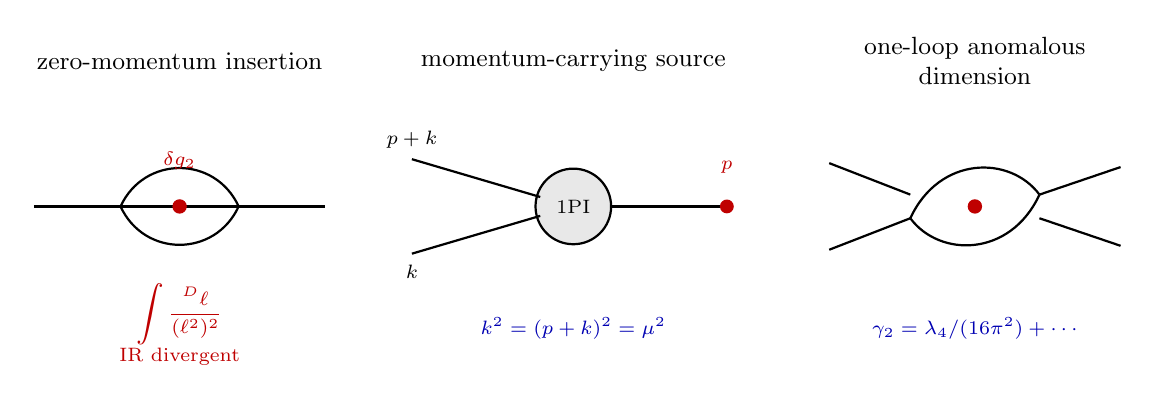
\begin{tikzpicture}[x=1cm,y=1cm,every node/.style={font=\scriptsize}]
    \begin{scope}
      \node[font=\small, align=center] at (0,2.55)
        {zero-momentum insertion};
      \draw[thick] (-1.85,0.7)--(1.85,0.7);
      \fill[red!75!black] (0,0.7) circle (2.6pt);
      \draw[thick] (-0.75,0.7)..controls (-0.45,1.35) and (0.45,1.35)..(0.75,0.7);
      \draw[thick] (-0.75,0.7)..controls (-0.45,0.05) and (0.45,0.05)..(0.75,0.7);
      \node[red!75!black, above] at (0,1.05) {\(\delta g_2\)};
      \node[align=center, red!75!black] at (0,-0.8)
        {\(\displaystyle\int\frac{\dd^D\ell}{(\ell^2)^2}\)\\IR divergent};
    \end{scope}

    \begin{scope}[shift={(5.0,0)}]
      \node[font=\small, align=center] at (0,2.55)
        {momentum-carrying source};
      \fill[gray!18, draw=black, thick] (0,0.7) circle (0.48);
      \node at (0,0.7) {1PI};
      \draw[thick] (-2.05,0.1)--(-0.42,0.58);
      \draw[thick] (-2.05,1.3)--(-0.42,0.82);
      \draw[thick] (0.48,0.7)--(1.95,0.7);
      \fill[red!75!black] (1.95,0.7) circle (2.5pt);
      \node[below] at (-2.05,0.08) {\(k\)};
      \node[above] at (-2.05,1.32) {\(p+k\)};
      \node[red!75!black, above] at (1.95,1.0) {\(p\)};
      \node[align=center, blue!70!black] at (0,-0.85)
        {\(k^2=(p+k)^2=\mu^2\)};
    \end{scope}

    \begin{scope}[shift={(10.1,0)}]
      \node[font=\small, align=center] at (0,2.55)
        {one-loop anomalous\\dimension};
      \draw[thick] (-1.85,0.15)--(-0.82,0.55);
      \draw[thick] (-1.85,1.25)--(-0.82,0.85);
      \fill[red!75!black] (0,0.7) circle (2.6pt);
      \draw[thick] (-0.82,0.55)..controls (-0.45,1.35) and (0.45,1.35)..(0.82,0.85);
      \draw[thick] (-0.82,0.55)..controls (-0.45,0.05) and (0.45,0.05)..(0.82,0.85);
      \draw[thick] (0.82,0.85)--(1.85,1.2);
      \draw[thick] (0.82,0.55)--(1.85,0.2);
      \node[blue!70!black, align=center] at (0,-0.85)
        {\(\gamma_2=\lambda_4/(16\pi^2)+\cdots\)};
    \end{scope}
  \end{tikzpicture}
  }
  \caption{The \(\phi^2\) operator is renormalized by coupling it to a source
  with nonzero momentum.  This avoids the infrared singularity of the
  zero-momentum subtraction and gives a finite definition of the anomalous
  dimension.}
  \label{fig:volume-ii-phi-two-renormalization}
\end{figure}

The one-loop source relation is
\[
  \delta\widetilde g_2(p;\mu)
  =
  \delta\widetilde g_2(p)
  \left[
    1
    -
    \frac{g_4}{2}
    \int
    \frac{\dd^{4-\epsilon}\ell}{(2\pi)^{4-\epsilon}}
    \frac{1}{\ell^2(p+\ell)^2}
    +
    O(g_4^2)
  \right],
\]
or
\[
  \delta\widetilde g_2(p;\mu)
  =
  \delta\widetilde g_2(p)
  \left[
    1
    -
    \frac{g_4}{2}
    (4\pi)^{-2+\epsilon/2}
    \frac{\Gamma(\epsilon/2)\Gamma(1-\epsilon/2)^2}{\Gamma(2-\epsilon)}
    |p|^{-\epsilon}
    +
    O(g_4^2)
  \right].
\]
It follows that
\[
  \gamma_2(\mu)
  =
  \lambda_4(\mu)
  \left(
    \frac{1}{16\pi^2}+O(\epsilon)
  \right)
  +
  O(\lambda_4(\mu)^2).
\]
At the Wilson-Fisher fixed point,
\[
  \gamma_{2*}
  =
  \frac{\epsilon}{3}+O(\epsilon^2),
  \qquad
  \Delta_{\phi^2}
  =
  (2-\epsilon)+\gamma_{2*}
  =
  2-\frac{2}{3}\epsilon+O(\epsilon^2).
\]

\section{Correlators and Local Composite Fields}

At the fixed point, the running of the renormalized momentum-space operator is
\[
  [\widetilde O_2(p)]_{\mu=|p|}
  =
  \left(\frac{|p|}{\mu_0}\right)^{-\gamma_{2*}}
  \widetilde O_2(p),
\]
where \(\mu_0\) is a fixed reference scale.  The correlator of renormalized
operators is finite and, by dimensional analysis,
\[
  \left\langle
    [\widetilde O_2(p)]_{\mu=|p|}
    [\widetilde O_2(q)]_{\mu=|q|}
  \right\rangle
  \propto
  \delta^{4-\epsilon}(p+q)\,|p|^{-\epsilon}.
\]
Consequently
\[
  \mu_0^{2\gamma_{2*}}
  \left\langle
    \widetilde O_2(p)\widetilde O_2(q)
  \right\rangle
  \propto
  \delta^{4-\epsilon}(p+q)\,|p|^{-\epsilon+2\gamma_{2*}}.
\]
Fourier transformation gives the position-space scaling law
\[
  \mu_0^{2\gamma_{2*}}
  \left\langle
    O_2(x)O_2(0)
  \right\rangle
  \propto
  \frac{1}{|x|^{2\Delta_{\phi^2}}},
  \qquad
  \Delta_{\phi^2}=2-\epsilon+\gamma_{2*}.
\]

\begin{figure}[H]
  \centering
  \resizebox{0.9\textwidth}{!}{%
  \begin{tikzpicture}[x=1cm,y=1cm,every node/.style={font=\scriptsize}]
    \node[draw=black, rounded corners, align=center, inner sep=6pt,
      minimum height=1.05cm] (renfinite)
      at (-4.2,0.9)
      {\(\displaystyle
      \langle[\widetilde O_2(p)]_{|p|}
      [\widetilde O_2(q)]_{|q|}\rangle\)\\
       \(\displaystyle\propto\delta(p+q)|p|^{-\epsilon}\)};
    \node[draw=black, rounded corners, align=center, inner sep=6pt,
      minimum height=1.05cm] (running)
      at (0.4,0.9)
      {\(\displaystyle
      [\widetilde O_2(p)]_{|p|}\)\\
      \(\displaystyle=(|p|/\mu_0)^{-\gamma_{2*}}\widetilde O_2(p)\)};
    \node[draw=black, rounded corners, align=center, inner sep=6pt,
      minimum height=1.05cm] (position)
      at (4.45,0.9)
      {\(\displaystyle
      \langle O_2(x)O_2(0)\rangle\)\\
       \(\displaystyle\propto |x|^{-2\Delta_{\phi^2}}\)};
    \draw[-{Latex[length=2mm]}, thick] (renfinite.east)--(running.west);
    \draw[-{Latex[length=2mm]}, thick] (running.east)--(position.west);
    \node[blue!70!black] at (0.4,-0.65)
      {\(\Delta_{\phi^2}=2-\epsilon+\gamma_{2*}\)};
  \end{tikzpicture}
  }
  \caption{Renormalized momentum-space correlators at the fixed point have no
  scale other than the external momentum.  Undoing the operator running gives
  the anomalous power in the bare operator correlator and hence the
  position-space scaling dimension.}
  \label{fig:volume-ii-phi-two-correlator-scaling}
\end{figure}

The notation \(O_2=\phi^2\) is a label for the renormalized local field in this
operator family; it is not a definition by an unregulated product at
coincident points.  A point-splitting representative has the form
\[
  \mu_0^{\gamma_{2*}}O_2(x)
  \propto
  \lim_{x'\to x}
  |x'-x|^{2\gamma_{\phi*}-\gamma_{2*}}
  \left[
    \hat\phi(x')\hat\phi(x)
    -
    \left\langle\hat\phi(x')\hat\phi(x)\right\rangle
  \right],
\]
where the subtraction removes the singular two-point function before the
coincident-point limit is taken.

\section{Descendants and Irrelevant Directions}

The cubic operator is not independent at the interacting fixed point.  The
equation of motion has the schematic operator consequence
\[
  O_3(x)=\phi^3(x)\propto\Box\phi(x),
\]
so \(O_3\) is an equation-of-motion descendant of \(O_1=\phi\).  Its dimension
is
\[
  \Delta_{\phi^3}
  =
  \Delta_\phi+2.
\]

The quartic operator \(O_4=\phi^4\) is instead the operator associated with
motion in the quartic-coupling direction.  A small source perturbation obeys
the linearized RG equation
\[
  \frac{\dd\,\delta g_4(\mu)}{\dd\log\mu}
  =
  \frac{\partial\beta(\lambda_4(\mu))}
       {\partial\lambda_4(\mu)}
  \,\delta g_4(\mu).
\]
Therefore
\[
  \gamma_{4*}
  =
  \left.
  \frac{\partial\beta(\lambda_4)}{\partial\lambda_4}
  \right|_{\lambda_4=\lambda_{4*}}
  =
  \epsilon+O(\epsilon^2),
\]
and
\[
  \Delta_{\phi^4}
  =
  4-\epsilon+\gamma_{4*}
  =
  4+O(\epsilon^2)
  >
  D.
\]
Thus \(\phi^4\) is irrelevant at the interacting fixed point.  This statement
is about perturbations around the fixed point; it is compatible with the fact
that the quartic interaction was needed to produce that fixed point.

\begin{figure}[H]
  \centering
  \resizebox{0.92\textwidth}{!}{%
  \begin{tikzpicture}[x=1cm,y=1cm,every node/.style={font=\scriptsize}]
    \begin{scope}
      \node[font=\small, align=center] at (0,2.35)
        {\(\phi^3\) as descendant};
      \node[draw=black, rounded corners, inner sep=6pt] at (-1.05,0.7) {\(\phi^3\)};
      \node[draw=black, rounded corners, inner sep=6pt] at (1.2,0.7) {\(\Box\phi\)};
      \draw[-{Latex[length=2mm]}, thick] (-0.45,0.7)--(0.55,0.7);
      \node[above] at (0.05,0.92) {EOM};
      \node[blue!70!black, align=center] at (0,-0.55)
        {\(\Delta_{\phi^3}=\Delta_\phi+2\)};
    \end{scope}

    \begin{scope}[shift={(5.9,0)}]
      \node[font=\small, align=center] at (0,2.35)
        {\(\phi^4\) as irrelevant direction};
      \fill[gray!18, draw=black, thick] (0,0.7) circle (0.5);
      \node at (0,0.7) {1PI};
      \foreach \a in {35,145,215,325} {
        \draw[thick] ({0.5*cos(\a)},{0.7+0.5*sin(\a)})
          --++({0.92*cos(\a)},{0.92*sin(\a)});
      }
      \fill[red!75!black] (0,1.58) circle (2.5pt);
      \draw[red!75!black, thick] (0,1.58)--(0,1.2);
      \node[red!75!black, above] at (0,1.84) {\(\delta g_4\)};
      \node[blue!70!black, align=center] at (0,-0.55)
        {\(\gamma_{4*}=\beta'(\lambda_*)=\epsilon+\cdots\)\\
         \(\Delta_{\phi^4}>D\)};
    \end{scope}
  \end{tikzpicture}
  }
  \caption{The cubic operator is an equation-of-motion descendant.  The quartic
  operator is independent, but its dimension is larger than \(D\) at the
  interacting fixed point, so changing its coefficient is an irrelevant
  deformation.}
  \label{fig:volume-ii-wilson-fisher-operator-spectrum}
\end{figure}

The low-lying scalar dimensions are summarized as follows:
\[
  \begin{array}{c|ccc}
    & \Delta_\phi & \Delta_{\phi^2} & \Delta_{\phi^4} \\
    \hline
    d=4-\epsilon
      & 1-\frac{\epsilon}{2}+O(\epsilon^2)
      & 2-\frac{2}{3}\epsilon+O(\epsilon^2)
      & 4+O(\epsilon^2) \\
    d=3
      & 0.518\ldots
      & 1.412\ldots
      & 3.829\ldots \\
    d=2
      & 0.125
      & 1
      & 4
  \end{array}
\]
The first row is the perturbative epsilon expansion.  The \(d=3\) and \(d=2\)
rows are data about the corresponding fixed points themselves; they are not
deduced by substituting \(\epsilon=1\) or \(\epsilon=2\) into the first-order
series.
